\chapter{O modelo de Lorenz 80 determinístico} \label{cap:ch01-lorenz-deterministico}

\section{Introdução - atualizar} \label{sec:ch01-introducao}
Este capítulo tem como objetivo apresentar o modelo determinístico Lorenz 80. Para isso, começamos, na seção \ref{sec:ch01-geofisica}, com uma introdução aos conceitos básicos de geofísica, a fim de familiarizar o leitor com os fundamentos dessa área. Em seguida, na seção \ref{sec:ch01-apresentacao-do-modelo}, contextualizamos o modelo, discutindo os trabalhos que o precederam e as motivações por trás de sua formulação.

Na seção \ref{sec:ch01-agua-rasa}, introduzimos o modelo de água rasa, que serve de base para o desenvolvimento do Lorenz 80. A construção deste é detalhada na seção \ref{sec:ch01-construcao-do-modelo}. Por fim, a seção \ref{sec:ch01-simulacoes-deterministico} traz simulações computacionais realizadas com o modelo, acompanhadas de uma análise gráfica dos resultados.

\section{Breves considerações sobre geofísica} \label{sec:ch01-geofisica}

Nesta seção, reunimos um breve glossário com os principais conceitos de geofísica que servem de base para a compreensão do modelo de Lorenz 80. Todas as definições expostas abaixo estão detalhadas em \citet{Vallis2017}.
\begin{itemize}
	\item \textbf{Convecção.} Convecção é um processo de transferência de calor que ocorre em
	      fluidos. Esse fenômeno envolve o movimento do próprio
	      fluido e a transferência energia térmica de uma região para outra.
	\item \textbf{Parâmetro de Coriolis.} A \textit{força de Coriolis} é uma quasi-força (ou pseudo-força) que surge devido à rotação da Terra. Quando analisamos o movimento de um corpo em um referencial rotativo, esse corpo parece sofrer a ação de uma força que desvia sua trajetória. Esse desvio é quantificado pelo parâmetro de Coriolis, definido pela expressão:
	      \begin{equation*}
	      	f = 2 \Omega \sin(\theta)
	      \end{equation*}
	      onde $\Omega$ representa a velocidade angular de rotação da Terra e $\theta$ é a latitude, ou seja, o ângulo entre a posição do ponto e o equador terrestre.
	      	      	      
	\item \textbf{Número de Rossby.} O número de Rossby é a razão entre a magnitude da aceleração relativa e a aceleração de Coriolis. É aproximado por:
	      \begin{equation*}
	      	Ro \equiv \frac{U}{fL},
	      \end{equation*}
	      	      	      
	      onde $U$ é a magnitude aproximada da velocidade horizontal e $L$ é uma escala de comprimento e $f$ é o parâmetro de Coriolis.
	      	      	      
	\item \textbf{Equilíbrio hidrostático.} Matematicamente, a equação do equilíbrio hidrostático é dada por:
	      \begin{equation}
	      	\frac{\partial p}{\partial z} = - \rho_0g, \label{eq:ch01-equilibrio-hidrostatico}
	      \end{equation}
	      	      	          
	      onde: $p$ é a pressão do fluido, $z$ é a coordenada vertical, $\rho_0$ é a densidade constante do fluido e $g$ é a aceleração da gravidade.
	\item \textbf{Conservação de massa.} Em um escoamento de fluido, a densidade pode variar de acordo com o tempo ou a posição. No entanto, a \textit{quantidade total de massa} do fluido permanece constante. Esse princípio estabelece que a massa não pode ser criada nem perdida durante o movimento.
	      	      	      
	\item \textbf{Equações quasi-geostróficas.} As equações quasi-geostróficas são equações  amplamente usadas em estudos teóricos da atmosfera e oceano. Elas atendem as seguintes características:
	      \begin{enumerate}
	      	\item O número de Rossby é pequeno;
	      	\item A escala do movimento não é significativamente maior do que a escala de deformação;
	      	\item As variações no parâmetro de Coriolis são pequenas;
	      	\item As escalas de tempo são advectivas, ou seja, $T=L/U$.
	      \end{enumerate}
	      
	\item \textbf{Condições de Hardley.} circulação de Hadley é um padrão atmosférico típico da região entre o Trópico de Câncer e o Trópico de Capricórnio. Nessa faixa tropical, o ar quente sobe próximo ao equador, se desloca em altitude para latitudes maiores e desce, formando um ciclo convectivo. As condições que regem este sistema, será utilizado em nossa simulação como as condições ideias da atmosfera, referida como ``condições de Hardley''.
\end{itemize}


\section{O modelo de água-rasa} \label{sec:ch01-agua-rasa}
O modelo de água rasa descreve um fluido de densidade constante, em equilíbrio hidrostático, que pode ou não estar em rotação. Nele, a escala horizontal é significativamente maior que a profundidade. Esse fluido possui superfície livre e é limitado pelas bordas \citep{Vallis2017}. No caso considerado, adotamos a versão de uma única camada.

Para a construção do modelo de água-rasa, consideramos a equação do equilíbrio hidrostático, expressa em \eqref{eq:ch01-equilibrio-hidrostatico}. A partir das manipulações envolvendo os conceitos de momento e conservação de massa, detalhado em \citet{Vallis2017}, obtemos as equações que descrevem o modelo: 
\begin{equation}\label{eq:ch01-agua-rasa}   
    \begin{aligned}
        \frac{\partial V}{\partial t} + (V \cdot \nabla)V + f \mathbf{k} \times V &= -g \nabla \eta \\
	    \frac{\partial \eta}{\partial t} + \nabla \cdot (\eta V)                  &= 0   
    \end{aligned}
\end{equation}
	    


Onde:
\begin{itemize}
	\item $t$: tempo;
	\item $\mathbf{r}$: vetor de posição inicial;
	\item $V(t)$: Velocidade horizontal;
	\item $\eta(t)$: altura da superfície;
	\item $\mathbf{k}$: vetor da vertical.
\end{itemize}

\section{Construção dos modelos} \label{sec:ch01-construcao-do-modelo}

Edward Norton Lorenz (1917-2008) foi um importante matemático e meteorologista responsável pela publicação de vários artigos com desenvolvimento de modelos na área de meteorologia e geofísica.

O mais famoso deles foi o artigo \textit{``Deterministic Nonperiodic Flow''}, publicado em 1963 \citet{Lorenz1963}. Nele, Lorenz desenvolveu um modelo matemático simplificado para a convecção atmosférica, composto por três equações diferenciais ordinárias, expressas abaixo:
\begin{align}
	\begin{cases}
	\frac{dx}{dt} & = \sigma(y-x)     \\
	\frac{dy}{dt} & = x(\rho - z) - y \\
	\frac{dz}{dt} & = xy - \beta z    
	\end{cases},
	\label{eq:ch01-lorenz63}
\end{align}

onde $\sigma$ é o \textit{número de Prandtl}, que regula a sensibilidade entre $x$ e $y$; $\rho$ é o \textit{número de Rayleigh}, associado à magnitude da convecção; e $\beta$ está ligado à geometria da célula de convecção, influenciando a relação entre as taxas de $x$ e $z$.
    
O modelo acima, conhecido como Lorenz 63, é um sistema determinístico desenvolvido para representar sistemas hidrodinâmicos ideais e dissipativos de força. O Lorenz 63 tornou-se amplamente conhecido por sua alta sensibilidade às condições iniciais — pequenas alterações nas variáveis $x_0$, $y_0$ e $z_0$ podem levar a trajetórias completamente distintas no espaço de fases. Essa sensibilidade extrema é uma característica caótica do modelo.

Em 1980, Lorenz publica o artigo intitulado ``\textit{Attractor Sets and Quasi-Geostrophic Equilibrium }'' \citep{Lorenz1980}. Neste artigo, Lorenz apresenta a construção e a simulação de dois modelos distintos: o primeiro, é formado a partir das equações primitivas (PE) com nove EDOs (equações diferenciais ordinárias), derivado das equações de águas rasas com topografia e forçamento, enquanto o segundo é um modelo quasi-geostrófico (QG) com 3 EDOs, obtido ao descartar as variáveis associadas ao escoamento divergente $x$ e seus termos correspondentes. O modelo PE contém tanto ondas gravitacionais rápidas quanto oscilações quasi-geostróficas lentas, enquanto o modelo QG mantém apenas estas últimas, em um quadro simplificado para atmosfera de latitudes médias. 

Por fim, o modelo BE (\textit{balanced equations}) foi introduzido em 1982 no artigo ``\textit{Intermediate Model Solutions to the Lorenz Equations: Strange Attractors and Other Phenomena}'' \citep{Gent1982} e é uma simplificação do modelo PE realizada através dos truncamentos das equações de vorticidade e divergência.

A seguir, apresentaremos a construção de cada um dos modelos apresentamos acima.

\subsection{Modelo PE}\label{sec:ch01-modelo-pe}
Consideremos um fluido homogêneo e incompressível, ou seja, com densidade constante em todo o volume e volume invariável mesmo sob variações de pressão. O escoamento é predominantemente horizontal, descrito por uma velocidade $V(t, \mathbf{r})$ independente da altura, onde $\mathbf{r}$ representa o vetor de posição inicial.

A componente vertical da velocidade é determinada pela continuidade de massa. A superfície livre do fluido está localizada na altura $H + z(t, \mathbf{r})$, onde $H$ representa a profundidade média e a base se apoia sobre uma topografia variável $h(\mathbf{r})$. Temos também que $h(\mathbf{r})$ e $z(t, \mathbf{r})$ possuem média zero.

O sistema está sujeito à rotação planetária, com um parâmetro de Coriolis constante $f$. 
Tanto o campo de velocidades $V$ quanto a elevação da superfície $z$ sofrem dissipação difusiva, 
associada a movimentos de pequena escala: o termo $\nu$ representa o coeficiente de difusão viscosa (dissipação de momento) e $\kappa$ representa o coeficiente de difusão térmica. O modelo também inclui um termo de forçamento externo $F(\mathbf{r})$ e, por fim, adota-se a hipótese de equilíbrio hidrostático.


A partir da descrição acima, podemos construir o seguinte diagrama:
\begin{figure}[htbp]
	\centering
	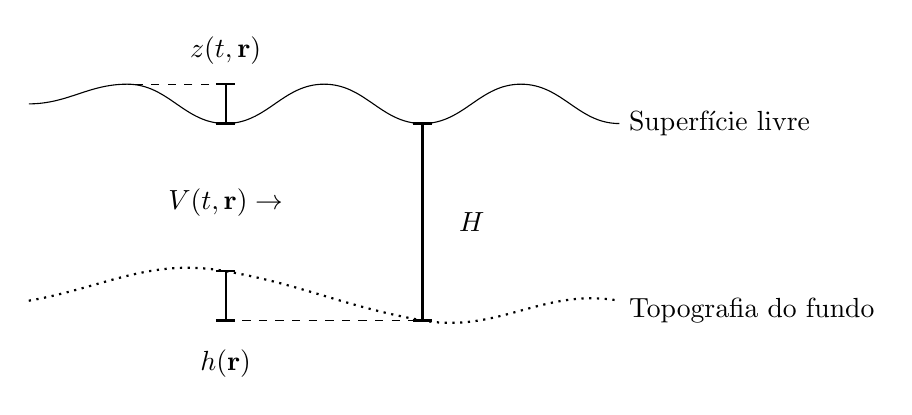
\begin{tikzpicture}[scale=1.25] 
										
		% Superfície livre
		\draw[above] (0,4) to[out=0,in=180] (1,4.2) 
		to[out=0,in=180] (2,3.8)
		to[out=0,in=180] (3,4.2)
		to[out=0,in=180] (4,3.8)
		to[out=0,in=180] (5,4.2)
		to[out=0,in=180] (6,3.8);
		\node[right] at (6,3.8) {Superfície livre};
										
		% Linha tracejada de referência para z
		\draw[dashed] (2,4.2) -- (1,4.2);
										
		% Desvio da superfície z
		\draw[thick] (2,3.8) -- (2,4.2);
		\draw[thick] (1.9,3.8) -- (2.1,3.8); 
		\draw[thick] (1.9,4.2) -- (2.1,4.2); 
		\node[above] at (2,4.3) {$z(t,\mathbf{r})$};
										
		% Velocidade V(t,r)
		\node at (2,3) {$ V(t,\mathbf{r}) \rightarrow$};
										
		% Profundidade média H
		\draw[thick] (4,3.8) -- (4,1.8);
		\draw[thick] (3.9,3.8) -- (4.1,3.8); 
		\draw[thick] (3.9,1.8) -- (4.1,1.8);
		\node at (4.5,2.8) {$H$};
										
		% Topografia do fundo (curva inferior)
		\draw[dotted, thick] (0,2) to[out=10,in=170] (2,2.3) 
		to[out=350,in=170] (4,1.8) 
		to[out=350,in=170] (6,2);
		\node[right] at (6,1.9) {Topografia do fundo};
										
		% Variação da topografia h
		\draw[thick] (2,2.3) -- (2,1.8);
		\draw[thick] (1.9,2.3) -- (2.1,2.3);
		\draw[thick] (1.9,1.8) -- (2.1,1.8); 
		\node[below] at (2,1.6) {$h(\mathbf{r})$};
										
		% Linha tracejada de referência para h
		\draw[dashed] (2,1.8) -- (4,1.8);
										
	\end{tikzpicture}
	\caption{Diagrama do modelo de água-rasa adaptado}
	\label{fig:fluido-topografia}
\end{figure}

Além disso, o modelo de água-rasa adaptado é expresso por:
\begin{align}
	\frac{\partial V}{\partial t} & = - ( V \cdot \nabla)V - f \mathbf{k} \times V - g \nabla z + \nu \nabla^2 V \label{eq:ch01-agua-rasa-modificada-1}     \\
	\frac{\partial z}{\partial t} & = - (V \cdot \nabla)(z - h) - (H + z - h)\nabla \cdot  V + \kappa \nabla^2 z + F \label{eq:ch01-agua-rasa-modificada-2} 
\end{align}

Onde:
\begin{itemize}
	\item $H$: profundidade média do fluido;
	\item $h(\mathbf{r})$: variação da superfície topológica;
	\item $V(t,\mathbf{r})$: Velocidade horizontal;
	\item $z(t,\mathbf{r})$: altura da superfície;
	\item $F$: forças externas;
	\item $\kappa$: coeficiente de difusão viscosa;
	\item $\nu$: coeficiente de difusão térmica;
\end{itemize}

Em seguida, aplicando o \textit{Teorema de Helmholtz} \footnote{O Teorema afirma que: ``Um vetor é unicamente determinado ao se conhecer sua divergência e seu rotacional
em uma região simplesmente conexa (sem buracos) e o seu componente normal sobre a fronteira'' \citep{Arfken2005}. A partir do Teorema, temos que campo vetorial suficientemente suave pode ser decomposto como
\begin{equation*}
    \mathbf{V} = \nabla \phi + \nabla \times \mathbf{A},
\end{equation*}
onde $\phi$ é o potencial escalar associado à divergência e $\mathbf{A}$ é o potencial vetorial associado ao rotacional. Também referido como \textit{decomposição de Helmholtz}.} à equação \eqref{eq:ch01-agua-rasa-modificada-1}, escrevendo
\begin{equation*}
	V = \nabla \chi + \mathbf{k} \times \nabla \psi,
\end{equation*}
onde $\chi$ é o potencial de velocidade associado à parte divergente e $\psi$ a função corrente associada à parte rotacional. Dessa forma, $\nabla^2 \chi$ representa a divergência e $\nabla^2 \psi$ a vorticidade. Substituindo essa decomposição obtemos:
\begin{align}
	\frac{\partial \nabla^2 \chi}{\partial t} & = -\tfrac{1}{2}\nabla^2(\nabla \chi \cdot \nabla \chi) 
	- \nabla \chi \cdot \nabla(\nabla^2\psi) \times \mathbf{k} 
	+ \nabla^2(\nabla \chi \cdot \nabla \psi \times \mathbf{k}) \nonumber \\
	                                          & \quad + \nabla \cdot (\nabla^2\psi\nabla\psi)          
	- \tfrac{1}{2}\nabla^2(\nabla \psi \cdot \nabla \psi) 
	+ \nu\nabla^4\chi + f\nabla^2\psi - g\nabla^2z, \label{eq:ch01-equacao-basica-1} \\
	\frac{\partial \nabla^2 \psi}{\partial t} & = -\nabla \cdot (\nabla^2\psi\nabla \chi)              
	- \nabla \psi \cdot \nabla(\nabla^2\psi) \times \mathbf{k} 
	- f\nabla^2\chi + \nu\nabla^4\psi. \label{eq:ch01-equacao-basica-2}
\end{align}

Analogamente, aplicando \eqref{eq:ch01-agua-rasa-modificada-2}, temos:
\begin{equation}
	\frac{\partial z}{\partial t} 
	= -\nabla \cdot \left[(z - h)\nabla \chi\right] 
	- \nabla \psi \cdot \nabla(z - h) \times \mathbf{k} 
	- H\nabla^2\chi + \kappa\nabla^2z + F. 
	\label{eq:ch01-equacao-basica-3}
\end{equation}

Nosso objetivo é reduzir as equações \eqref{eq:ch01-equacao-basica-1}–\eqref{eq:ch01-equacao-basica-3} a um modelo de baixa ordem. Para isso, introduzimos três vetores adimensionais $\alpha_1, \alpha_2, \alpha_3$ que satisfazem
\begin{equation*}
	\alpha_1 + \alpha_2 + \alpha_3 = 0,
\end{equation*}
e adotamos as permutações cíclicas
\begin{equation}
	(i,j,k) = (1,2,3),\; (2,3,1),\; (3,1,2).
\end{equation}\label{eq:ch01-permutacoes}
Definimos então:
\begin{equation*}
	a_i = \alpha_i \cdot \alpha_i, 
	\quad b_i = \alpha_j \cdot \alpha_k, 
	\quad c = (b_1b_2+b_2b_3+b_3b_1)^{1/2}.
\end{equation*}

Lorenz também apresenta uma forma alternativa, equivalente, mais conveniente para a implementação computacional:
\begin{equation*}
	b_i = \tfrac{1}{2}(a_i - a_j - a_k), 
	\quad c_i = c.
\end{equation*}

Escolhido um comprimento característico $L$, construímos três funções ortogonais:
\begin{equation*}
	\phi_i(\mathbf{r}) = \cos\!\left(\alpha_i \cdot \frac{\mathbf{r}}{L}\right),
\end{equation*}
para as quais valem, por exemplo:
\begin{align*}
	L^2\nabla^2\phi_i                              & = -a_i\phi_i,                         \\
	L^2\nabla\phi_i \cdot \nabla\phi_k             & = -\tfrac{1}{2}b_{ik}\phi_i + \cdots, \\
	L^2\nabla \cdot (\phi_j\nabla\phi_k)           & = \tfrac{1}{2}b_{jk}\phi_i + \cdots,  \\
	L^2\phi_j \cdot \nabla\phi_k \times \mathbf{k} & = -\tfrac{1}{2}c_{jk}\phi_i + \cdots, 
\end{align*}
onde os termos omitidos são múltiplos de cossenos. Com essas funções, expandimos as variáveis em série e introduzimos escalas adimensionais:
\begin{equation}\label{eq:ch01-adimensionalizacao}
	\begin{aligned}
		t    & = f^{-1}\tau,                     \\
		\chi & = 2L^2f^2 \sum_i x_i\phi_i,       \\
		\psi & = 2L^2f^2 \sum_i y_i\phi_i,       \\
		z    & = 2L^2f^2g^{-1} \sum_i z_i\phi_i, \\
		h    & = 2L^2f^2g^{-1} \sum_i h_i\phi_i, \\
		F    & = 2L^2f^2g^{-1} \sum_i F_i\phi_i. 
	\end{aligned}
\end{equation}

Substituindo as equações de \eqref{eq:ch01-adimensionalizacao} em \eqref{eq:ch01-equacao-basica-1}–\eqref{eq:ch01-equacao-basica-3}, e projetando sobre a base $\{\phi_i\}$, obtemos finalmente o modelo PE de baixa ordem, composto de nove equações diferenciais ordinárias:
\begin{align}
	a_i\frac{dx_i}{d\tau} & = a_ib_ix_ix_k - c(a_i - a_k)x_iy_k      
	+ c(a_i - a_j)y_ix_k -2c^2y_iy_k - \nu_0a_i^2x_i + a_iy_i - a_iz_i, \label{eq:ch01-modelo-pe-1}\\
	a_i\frac{dy_i}{d\tau} & = -a_ib_kx_iy_k - a_ib_iy_ix_k           
	+ c(a_k - a_i)y_iy_k - a_ix_i - \nu_0a_i^2y_i, \label{eq:ch01-modelo-pe-2}\\
	\frac{dz_i}{d\tau}    & = -b_kx_i(z_k - h_k) - b_i(z_i - h_i)x_k 
	+ c\,y_i(z_k - h_k) - c(z_i - h_i)y_k + g_0a_ix_i - \kappa_0a_iz_i + F_i. \label{eq:ch01-modelo-pe-3}
\end{align}

As variáveis $x_i$ representam os modos divergentes do escoamento, associados às ondas de gravidade; as variáveis $y_i$ correspondem aos modos rotacionais (vorticidade), ligados às oscilações quasi-geostróficas; e as variáveis $z_i$ funcionam como variáveis auxiliares acopladas ao sistema. Na classificação em relação à variáveis rápidas e lentas, temos que: $x_i$ corresponde as variáveis rápidas, enquanto $y_i$ e $z_i$ correspondem as variáveis lentas.

\subsection{O modelo QG}\label{sec:ch01-modelo-qg}
Na construção do modelo QG, começamos desprezando todos os termos não lineares, assim como aqueles que envolvem as variáveis $x$, incluindo a derivada temporal, na equação \eqref{eq:ch01-modelo-pe-1}. Fazemos o mesmo com os termos não lineares ou topográficos que dependem de $x$ nas equações \eqref{eq:ch01-modelo-pe-2} e \eqref{eq:ch01-modelo-pe-3}. Por fim, eliminamos as variáveis $x$ e $z$, obtendo ao modelo QG apresentado a seguir:
\begin{equation}
	(a_i g_0 + 1)\,\frac{dy_i}{d\tau} 
	= g_0 c (a_k - a_j) y_j y_k 
	- a_i (a_i g_0 \nu_0 + \kappa_0) y_i 
	- c h_k y_j + c h_j y_k + F_i,
	\label{eq:ch01-modelo-lorenz-deterministico-qg}
\end{equation}
onde ainda são válidas as permutações apresentadas em \eqref{eq:ch01-permutacoes}.

\subsection{O modelo BE}\label{sec:ch01-modelo-be}
Como afirmado anteriormnte, o modelo BE baseia-se em truncamentos das equações de vorticidade e divergência. No caso, na equação de vorticidade, o termo omitido é um termo de advecção vertical de modo que a equação de vorticidade e a equação de altura são exatas. No nosso caso, o truncamento é aplicado em \eqref{eq:ch01-modelo-pe-2} e \eqref{eq:ch01-modelo-pe-3}, resultando na expressão:
\begin{equation}
    a_i y_i - 2c^2 y_j y_k = a_i z_i .
\end{equation}\label{eq:ch01-truncamento-be}

Derivando a expressão acima, obtemos:
\begin{equation*}
    a_i \left( \frac{dy_i}{d\tau} - \frac{dz_i}{d\tau} \right) -2c^2 \left( \frac{dy_j}{d\tau} y_k + y_j \frac{dy_k}{d\tau} \right) = 0
\end{equation*}

Aplicando em \eqref{eq:ch01-modelo-pe-2} e \eqref{eq:ch01-modelo-pe-3}, obtemos:
\begin{equation}
    \begin{aligned}
        x_i &[\, a_i a_j a_k (1 + g_0 a_i)
        - 2c^2 (a_j^2 b_j y_j^2 + a_k^2 b_k y_k^2) \,]\\
        &- x_j [\, a_j a_k (y_k (2c^2 - a_k b_k) + a_j b_k (z_k - h_k)) + 2c^2 a_i b_j \dot{y_j} y_j \,]\\
        &- x_k [\, a_i a_j a_k (y_j (2c^2 - a_j b_j) + a_i b_j (z_j - h_j)) + 2c^2 a_i b_k \dot{y_k} y_k \,]\\
        &= a_j a_k [\, c (a_k - a_j) y_j y_k + c a_i ((z_j - h_j) y_k - y_j (z_k - h_k)) \,]\\
        &\quad + a_i (v_0 a_i (z_i - y_i) - F_i)\\
        &\quad - 2c^2 [\, c a_j (a_j - a_i) y_j y_j^2 + c a_k (a_i - a_k) y_k y_k^2 \,]\\
        &\quad - v_0 a_j a_k (a_j + a_k) y_j y_k .
    \end{aligned}
\end{equation}\label{eq:ch01-modelo-be-equacao}

Novamente, assim como no caso anterior, ainda são válidas as permutações apresentadas em \eqref{eq:ch01-permutacoes}.

Podemos representar de forma mais clara e compacta com o uso da função $\Phi(y)$, proposta em \citet{Chekroun2017}, expressa por:
\begin{equation}
    \Phi(\mathbf{y}) = (\Phi_1(\mathbf{y}), \, \Phi_2(\mathbf{y}), \, \Phi_3(\mathbf{y}))
    = \left[ M(\mathbf{y}, G(\mathbf{y})) \right]^{-1}
    \begin{pmatrix}
        d_{1,2,3}(\mathbf{y}, G(\mathbf{y})) \\
        d_{2,3,1}(\mathbf{y}, G(\mathbf{y})) \\
        d_{3,1,2}(\mathbf{y}, G(\mathbf{y}))
    \end{pmatrix}.
\end{equation}\label{eq:ch01-phi-be}

onde,
\begin{equation*}
    M(\mathbf{y}, \mathbf{z}) \mathbf{x} =
    \begin{pmatrix}
        \Delta_{1,2,3}(\mathbf{y}) & \Gamma_{1,2,3}(\mathbf{y}, \mathbf{z}) & \Sigma_{1,2,3}(\mathbf{y}, \mathbf{z}) \\
        \Sigma_{2,3,1}(\mathbf{y}, \mathbf{z}) & \Delta_{2,3,1}(\mathbf{y}) & \Gamma_{2,3,1}(\mathbf{y}, \mathbf{z}) \\
        \Gamma_{3,1,2}(\mathbf{y}, \mathbf{z}) & \Sigma_{3,1,2}(\mathbf{y}, \mathbf{z}) & \Delta_{3,1,2}(\mathbf{y})
    \end{pmatrix}
    \begin{pmatrix}
        x_1 \\x_2 \\x_3
    \end{pmatrix}
    =
    \begin{pmatrix}
        d_{1,2,3}(\mathbf{y}, \mathbf{z}) \\
        d_{2,3,1}(\mathbf{y}, \mathbf{z}) \\
        d_{3,1,2}(\mathbf{y}, \mathbf{z})
    \end{pmatrix}.
\end{equation*}

com
\begin{align*}
    \Delta_{i,j,k}(\mathbf{y})
    &= a_i a_j a_k (1 + g_0 a_i)
     - 2c^2 \left( a_j^2 b_j y_j^2 + a_k^2 b_k y_k^2 \right),\\
    \Gamma_{i,j,k}(\mathbf{y}, \mathbf{z})
    &= -\left[ a_j a_k \left( y_k (2c^2 - a_k b_k) + a_j b_k (z_k - h_k) \right)
     + 2c^2 a_i b_j \dot{y_j} y_j \right],\\
    \Sigma_{i,j,k}(\mathbf{y}, \mathbf{z})
    &= -\left[ a_i a_j \left( y_j (2c^2 - a_j b_j) + a_i b_j (z_j - h_j) \right)
     + 2c^2 a_i b_k \dot{y_k} y_k \right],\\
    d_{i,j,k}(\mathbf{y}, \mathbf{z})
    &= a_j a_k \left[ c (a_k - a_j) y_j y_k + c a_i ((z_j - h_j) y_k - y_j (z_k - h_k)) \right]\\
    &\quad + a_i (v_0 a_i (z_i - y_i) - F_i)\\
    &\quad - 2c^2 \left[ c a_j (a_j - a_i) y_j y_j^2 + c a_k (a_i - a_k) y_k y_k^2 \right]\\
    &\quad - v_0 a_j a_k (a_j + a_k) y_j y_k .
\end{align*}

Assim, a equação \eqref{eq:ch01-modelo-be-equacao}, pode ser expressa por:
\begin{equation*}
    a_i \frac{dy_i}{d\tau}
= -a_k b_k \Phi_j(\mathbf{y}) y_k
  - a_j b_j y_j \Phi_k(\mathbf{y})
  + c (a_k - a_j) y_j y_k
  - a_i \Phi_i(\mathbf{y})
  - v_0 a_i^2 y_i .
\end{equation*}
\newpage
\section{Simulações} \label{sec:ch01-simulacoes-deterministico}
Nesta seção, expor os resultados gráficos das simulações do Lorenz 80 determinístico com o objetivo de apresentar ao leitor o comportamento do modelo visualmente, bem como exibir características e propriedades de cada modelo. Para as simulações utilizamos a linguagem \textit{Python}, em particular, bibliotecas \textit{scipy}, \textit{numpy} e \textit{pandas}. O código utilizado está no apêndice \ref{app_sec:lorenz80-det}. Os parâmetros utilizados estão de acordo com \citet{Lorenz1980} e \citet{Chekroun2021}, são: $\kappa = \nu = \frac{1}{48}$, $g_0 = 8 \text{ m} \cdot \text{s}^{-2}$, $a_1 = a_2 = 1$, $a_3 =3$, $h_1 = -1$ e $h_2 = h_3 = f_2 = f_3 = 0$. Em relação a $f_1$, testamos com dois valores $f_1=0.1$ e $f_1=0.3027$ que estão devidamente enunciados quando utilizados.

\subsection{Simulações do modelo PE}
Tomando $f_1 = 0.1$ e $x = y = z = (0.1, 0.1, 0.1)$. Para tais valores, obtivemos os seguintes resultados:
\begin{figure}[H]
    \centering

    \begin{subfigure}{0.48\textwidth}
        \centering
        \includegraphics[width=\textwidth]{00_TCC/01_LATEX/figuras/ch01_lorenz_80/f01d01_cond_default.png}
        \caption{Evolução das variáveis $x_1, y_1, z_1$ em 1 dia}
        \label{fig:ch01-f01d01}
    \end{subfigure}
    \hfill
    \begin{subfigure}{0.48\textwidth}
        \centering
        \includegraphics[width=\textwidth]{00_TCC/01_LATEX/figuras/ch01_lorenz_80/f01d50_cond_default.png}
        \caption{Evolução das variáveis $x_1, y_1, z_1$ em 50 dias}
        \label{fig:ch01-f01d50}
    \end{subfigure}

    \caption{Evolução temporal das variáveis $x_1, y_1, z_1$}
    \label{fig:ch01-f01t}
\end{figure}

Inicialmente, no primeiro dia de simulação (figura \ref{fig:ch01-f01d01}), observa-se que a variável $x_1$ apresenta amplitude superior à de $y_1$, mas inferior à de $z_1$. Além disso, seu período é ligeiramente menor que o das demais variáveis. Esse comportamento reflete a natureza de $x_1$ como uma variável rápida, associada às oscilações do tipo onda gravitacional.

Na figura \ref{fig:ch01-f01d50}, após 50 dias de simulação, nota-se uma redução significativa da amplitude de $x_1$, acompanhada por oscilações mais rápidas e de menor intensidade. Isso é consistente com a dissipação progressiva das ondas gravitacionais, um efeito esperado devido à presença de termos dissipativos no modelo.

Com relação às variáveis lentas $y_1$ e $z_1$, percebe-se na figura \ref{fig:ch01-f01d01} que $z_1$ possui a maior amplitude, enquanto $y_1$ apresenta a menor. Ambas têm períodos semelhantes. Já na figura \ref{fig:ch01-f01d50}, observa-se que $y_1$ e $z_1$ passam a exibir comportamento oscilatório sincronizado, com amplitudes mais próximas. Esse acoplamento dinâmico evidencia a convergência das trajetórias do sistema para o atrator, que no contexto do modelo. Essa convergência e sincronização indicam que, ao longo do tempo, a solução do sistema se aproxima de um regime dominado por oscilações de baixa frequência e mais regulares enquanto as componentes associadas a modos rápidos (como $x_1$) são dissipadas \citep{Lorenz1980}. Para as projeções bidimensionais, utilizamos $f_1=0.3027$ e as variáveis iniciais com as condições de Hardley expressas matematicamente abaixo:

\begin{equation}
	y_1 = \frac{f_1}{a_1 \nu_0 \cdot (1+a_1 g_0)}, \quad
	x_1 = -\nu_0a_1y_1 \quad \text{e} \quad 
	z_1 = y_1 \label{ch01-cond-hardley}
\end{equation}

Além disso, adicionamos pequenas pertubações em $y_2$ e $z_2$, $y_2 = -1\times 10^{-5}$ e $z_2 = 1\times 10^{-5}$ e variáveis foram fixadas em zero. As simulações foram realizadas ao longo de $400$ dias, sendo descartados os $25\%$ iniciais dos dados, correspondentes à fase transitória em que o sistema ainda está evoluindo até se ajustar ao formato do atrator. Assim, obtiveram-se os seguintes resultados:
\begin{figure}[htbp]
    \centering

    \begin{subfigure}{0.6\textwidth}
        \centering
        \includegraphics[width=\textwidth]{00_TCC/01_LATEX/figuras/ch01_lorenz_80/PE/pe_y3y2.png}
        \caption{Projeção no plano $(y_3, y_2)$.}
        \label{fig:ch01-pe-y3-y2}
    \end{subfigure}

    \begin{subfigure}{0.6\textwidth}
        \centering
        \includegraphics[width=\textwidth]{00_TCC/01_LATEX/figuras/ch01_lorenz_80/PE/pe_y1y2.png}
        \caption{Projeção no plano $(y_1, y_2)$.}
        \label{fig:ch01-pe-y1-y2}
    \end{subfigure}

    \begin{subfigure}{0.6\textwidth}
        \centering
        \includegraphics[width=\textwidth]{00_TCC/01_LATEX/figuras/ch01_lorenz_80/PE/pe_y1y3.png}
        \caption{Projeção no plano $(y_1, y_3)$.}
        \label{fig:ch01-pe-y1-y3}
    \end{subfigure}

    \caption{Projeções do modelo PE para $f_1 = 0.3027$.}
    \label{fig:ch01-pe-proj}
\end{figure}

O principal objetivo destas simulações projetadas bidimensionalmente é evidenciar o comportamento de atrator caótico característico do sistema. Note que, através da imagem, pode-se evidenciar a aperiodicidade do sistema, junto com o fato de que não há um ponto de convergência quando $t \to \infty$. Por fim, ponto importante é que as trajetórias permanecem confinadas em uma região limitada do espaço de fases, não divergindo para o infinito, caracterizando o atrator. 

\subsection{Simulações do modelo QG}

Para as simulações do modelo QG, utilizamos as mesmas condições utilizadas para as projeções do modelo PE, isto é, $f=0.3027$ e as condições de Harley para a variável $y_1$ expressa em \eqref{ch01-cond-hardley} e uma pequena pertubação em $y_2= 1 \times 10^{-5}$. Simualação com $t$ em $400$ dias e com limpeza de dados de $25\%$. 
\begin{figure}[htbp]
    \centering

    \begin{subfigure}{0.6\textwidth}
        \centering
        \includegraphics[width=\textwidth]{00_TCC/01_LATEX/figuras/ch01_lorenz_80/QG/qg_y3y2.png}
        \caption{Projeção no plano $(y_3, y_2)$.}
        \label{fig:ch01-qg-y3-y2}
    \end{subfigure}

    \begin{subfigure}{0.6\textwidth}
        \centering
        \includegraphics[width=\textwidth]{00_TCC/01_LATEX/figuras/ch01_lorenz_80/QG/qg_y1y2.png}
        \caption{Projeção no plano $(y_1, y_2)$.}
        \label{fig:ch01-qg-y1-y2}
    \end{subfigure}

    \begin{subfigure}{0.6\textwidth}
        \centering
        \includegraphics[width=\textwidth]{00_TCC/01_LATEX/figuras/ch01_lorenz_80/QG/qg_y1y3.png}
        \caption{Projeção no plano $(y_1, y_3)$.}
        \label{fig:ch01-qg-y1-y3}
    \end{subfigure}

    \caption{Projeções do modelo QG para $f_1 = 0.3027$.}
    \label{fig:ch01-qg-proj}
\end{figure}

Nas projeções mostradas nas Figuras \ref{fig:ch01-qg-y3-y2}–\ref{fig:ch01-qg-y1-y2}, percebe-se a formação de trajetórias regulares e confinadas, indicando uma forte correlação entre as variáveis $y_i$. Além disso, o modelo QG apresenta um regime visivelmente mais organizado. Ainda assim, o sistema mantém comportamento caótico: não há convergência para um ponto fixo quando $t \to \infty$, e o regime estacionário exibe um atrator estranho.


\subsection{Simulações do modelo BE}
Para o modelo BE, utilizamos os mesmos parâmetros e condições iniciais utilizadas nas projeções dos modelos anteriores, ainda com $400$ dias e $25\%$ dos dados iniciais eliminados.
\begin{figure}[htbp]
    \centering

    \begin{subfigure}{0.6\textwidth}
        \centering
        \includegraphics[width=\textwidth]{00_TCC/01_LATEX/figuras/ch01_lorenz_80/BE/be_y3y2.png}
        \caption{Projeção no plano $(y_3, y_2)$.}
        \label{fig:ch01-be-y3-y2}
    \end{subfigure}

    \begin{subfigure}{0.6\textwidth}
        \centering
        \includegraphics[width=\textwidth]{00_TCC/01_LATEX/figuras/ch01_lorenz_80/BE/be_y1y2.png}
        \caption{Projeção no plano $(y_1, y_2)$.}
        \label{fig:ch01-be-y1-y2}
    \end{subfigure}

    \begin{subfigure}{0.6\textwidth}
        \centering
        \includegraphics[width=\textwidth]{00_TCC/01_LATEX/figuras/ch01_lorenz_80/BE/be_y1y3.png}
        \caption{Projeção no plano $(y_1, y_3)$.}
        \label{fig:ch01-be-y1-y3}
    \end{subfigure}

    \caption{Projeções do modelo BE para $f_1 = 0.3027$.}
    \label{fig:ch01-be-proj}
\end{figure}

Visualmente, temos que o modelo BE, assim como os dois modelos anteriores, não há convergência quando $t \to \infty$, e o regime estacionário exibe um atrator estranho. Ao comparar aos modelos anteriores, temos que o modelo BE é muito semelhante ao modelo BE e, consequentemente, apresenta um comportamento mais comportato ao comparar com o modelo QG. 

Apesar das semelhanças entre os modelos BE e QG, observam-se diferenças nas escalas das variáveis $y$. Ao comparar as projeções $(y_3,y_2)$ e $(y_1,y_3)$ (Figs. \ref{fig:ch01-qg-y3-y2} vs. \ref{fig:ch01-be-y3-y2} e \ref{fig:ch01-qg-y1-y3} vs. \ref{fig:ch01-be-y1-y3}), verifica-se que as trajetórias do modelo QG ocupam uma região ligeiramente menor no plano de fases. 

Essa diferença reflete-se nas amplitudes das variáveis, conforme resumido na Tabela \ref{tab:amplitude-pe-qg-be}. As componentes $y_1$ e $y_2$ apresentam amplitudes ligeiramente menores no modelo QG, enquanto a variável $y_3$ exibe o comportamento oposto, com amplitude superior no modelo QG.

\begin{table}[H]
    \centering
    \caption{Comparação das amplitudes para cada modelo.}
    \label{tab:amplitude-pe-qg-be}
    \begin{tabular}{lccc}
        \toprule
        \textbf{Modelo} & $\boldsymbol{\Delta y_1}$ & $\boldsymbol{\Delta y_2}$ & $\boldsymbol{\Delta y_3}$ \\
        \midrule
        PE & 2.24 & 2.57 & 0.97 \\
        QG & 1.95 & 1.95 & 0.47 \\
        BE & 1.99 & 2.11 & 0.30 \\
        \bottomrule
    \end{tabular}
\end{table}

Também podemos verificar tal diferença de amplitude das variáveis $y$ na próxima imagem:
\begin{figure}
    \centering
    \includegraphics[width=\linewidth]{00_TCC/01_LATEX/figuras/ch01_lorenz_80/amplitudes.png}
    \caption{Comparação de amplitudes de $y$ para cada modelo}
    \label{fig:ch01-amplitudes}
\end{figure}
